\documentclass[10pt,a4paper]{article}
\usepackage[utf8]{inputenc}
\usepackage[english]{babel}
\usepackage{amsmath}
\usepackage{amsfonts}
\usepackage{amssymb}
\usepackage{hyperref}
\usepackage{graphicx}
\usepackage{caption}
\usepackage{subcaption}
\usepackage{color}
%
\graphicspath{ {../data/plots/} }
%
% \todo{} command.
% Usage: \todo{Document the TODO command.}
% Comment out second line to disable.
\newcommand{\todo}[1]{}
\renewcommand{\todo}[1]{{\color{red} TODO: {#1}} \\}
%
\newcommand{\AND}{\ensuremath{~AND~}}
\newcommand{\XOR}{\ensuremath{~XOR~}}
%
\author{Christian Bobach, 20104256}
\title{AMD tag overhead in a MPC outsourcing environment}
\begin{document}
\maketitle

\begin{abstract}
%\todo{WRITE abstract}
In this paper I argue through experiments that the addition of an algebraic manipulation detection code to the secure multiparty computation framework proposed in the paper \cite{fosc} is minimal. This has been done using a framework for secure evaluation of circuit in a two party setting. The evaluation has been done on different size circuit to see the development in the overhead added by the manipulation detection code.

The conclusion of the experiments is that the added overhead of the manipulation detection code is small. This is mainly because the places where the manipulation detection code generates the most overhead is not where the evaluation uses the most time. Therefor on large circuits the overhead of the added manipulation detection code is negligible.
\end{abstract}

\tableofcontents
\pagebreak

%INTRODUCTION
%papers, problem, solutions, introduction to experiments
\section{Introduction}
In this paper I have studied the framework proposed in \cite{fosc} and made experiments to measure the overhead added to the computation by securing the input and output with an algebraic manipulation detection(AMD) code.

%\todo{Introduction to paper \cite{fosc}}
In the paper they propose a framework for outsourcing secure multiparty computation(MPC) between any number of clients and workers with minimal overhead. The framework ensures input privacy is preserved and that the output is correct. This is done independent of the underlying MPC protocol. Their solution minimize the work needed done by the client, while they try to minimize the overhead on the workers. For correctness of output from the framework it is enough for one client to trust only one worker. This has the effect that the framework is not ensured to terminate as one worker can deadlock the system. They propose a way to detect a dishonest worker and as a solution not to use that worker for future computations. In this paper the focus will be on ensuring that the workers can not cheat by adding an error to the input of the client.

%\todo{Introduction to problem and solution}
Because the workers has the possibility to add an error $\epsilon$ to the input of a client or the output of the computation, there is a need for a way to ensure the detection of such an error. In the paper they propose the usage of an AMD code to ensure that a worker cannot create an variable tag $\tilde{t}=Tag(\tilde{k},\tilde{x})$ where $\tilde{t}=t+\epsilon_t$, $\tilde{k}=k+\epsilon_k$ and $\tilde{x}=x+\epsilon_x$. If this is possible a corrupted worker could chose $\tilde{x}$ and create a matching $\tilde{t}$ such that the protocol will output an incorrect result for the computation. This problem is exactly what the AMD code can overcome.

Before the workers output the secret share of the function computed they make an integrity check of the tag. A corrupted worker cannot change its share of the tag without breaking the security, and thereby terminating the execution. This will reveal the corrupted worker and therefore will this worker not be used in future computations. 

%\todo{Introduction to experiment}
It is the overhead of the added AMD code that I have studied in this paper. In the paper they state that the overhead is minimal. I have through experiments found an approximation of what the cost of the added AMD code is.

\bigskip
In the next section I will describe how the experiments was done, how the circuits was constructed and what that gave of results.

%EXPERIMENT
%what have we covered
%what is the hypothesises
%what is the results
\section{Experiment}
In this project I have used a framework called duplo\footnote{Duplo is an ongoing Ph.d. project by Roberto Trifiletti which is not public at the time of writing.} which is a framework for doing multiparty computations in a two party setting. The framework is used to construct the two parties communicating in the calculation. The framework gives the possibility to time the communication in the different phases. The two parties runs through six different phases during the execution. The six phases are as follows; setup, preprocess, solder, prepare, evaluate and decode. After these phases the parties hold the output computed based on their input and the circuit of the computation desired.

%\todo{How was the experiemnts done}
The experiments in this paper is done using a composed circuit as the computation. In the experiment I used two different composed circuit as inputs. Both of these consisting of multiple sub-circuits. The first composed circuit we will call $C_{ITA}$ consists of an ID-, a TAG- and a variable number of AES-circuits. The other composed circuit we will call $C_{IA}$ consists of an ID-circuit and a variable number of AES-circuits. The TAG-circuit will be denoted $C_{T}$. In the framework it is not possible to time the different sub-circuits of the composed circuit. Therefore both $C_{ITA}$ and $C_{IA}$ is run multiple times to get an average of the execution time with and without $C_{T}$. From this we can get an estimate of how much time is used on the $C_{T}$ by calculating $C_{ITA}-C_{IA}$. When we have the time for the $C_{T}$ it is easy to get the fraction of the time is used on $C_{T}$ compared to $C_{ITA}$ by calculating $\frac{C_{T}}{C_{ITA}}$. This allow us to figure out how much time $C_{T}$ adds of overhead. Thereby we get an idea of how big a circuit should be before we can neglect the overhead added by the AMD tag proposed in \cite{fosc}.

Before the experiments could begin I needed to construct $C_I$ and $C_T$ that should be used to make $C_{ITA}$. In the following sections I will introduce these circuits and why they were needed.

\subsection{Circuits}
First of all the duplo framework had an AES-circuit $C_A$, that could be used as the computation function. I needed to construct $C_I$ and $C_T$ before I could do the experiments. By using multiple $C_A$ as the variable size computation I could construct a :big computation" to measure the overhead added by $C_T$. By "the big computation" is meant, a computation that could give an idea of when $C_{T}$ could be negligible. The $C_I$, $C_T$ and $C_A$'s was soldered together to form $C_{ITA}$ that could be timed in the framework.

\bigskip
The input circuits was encoded using a modification of Nigel Smart's\footnote{Nighel's encoding can be found here: \url{https://www.cs.bris.ac.uk/Research/CryptographySecurity/MPC/}} circuit encoding that was used in the framework. To generate the circuits I used a modified version of the Fariplay circuit generator tool\footnote{The circuit generator can be found here: \url{https://github.com/cbobach/circuit-generator}} that has been used to convert circuits for the tiny MPC framework.

\bigskip
In the cumming section I will introduce the circuits I have constructed. First of all the $C_T$ that match the requirements from the paper. After that I will introduce $C_I$ and why that was needed.

\subsubsection{TAG-circuit}
\label{tag-circuit}
$C_T$ is made such that it meets the requirements for the tag proposed in \cite{fosc}.

%\todo{Security of the tag: do the math}
Doing the math for $C_T$ shows that input correctness is preserved and ensures that a malicious worker can not cheat and will be detected. Assuming that $x,k,s\not=0$ then a worker can not construct $t'=t$ successfully. Assume that it should be possible to construct $t'=t$ then it must be the case that $t=xk=(x+\epsilon_x)(k+\epsilon_k)=t'$. This implies that $x\epsilon_k+k\epsilon_x+\epsilon_x\epsilon_k=0$. Since $x,k\not=0$ then there are four different cases for $\epsilon_x$ and $\epsilon_k$; one where $\epsilon_x=1$ and $\epsilon_k=0$ which implies that $k=0$ this is a contradiction to the assumption that $k\not=0$. We reach a similar contradiction if $\epsilon_x=0$ and $\epsilon_k=1$. For the last interesting case where both $\epsilon_x,\epsilon_k=1$ we have that $x+k+1=0$. Since the calculation is done on bits we have that either $x=1$ or $k=1$ and that $x+k=1$. This implies that either $x=0$ or $k=0$. This is a contradiction to the assumption and therefore it can only be the case that both $\epsilon_x,\epsilon_k=0$ which clearly satisfies the condition that $t=xk=(x+0)(k+0)=t'$. This is okay since it reflects that the input was not changed in any way.
This ensures the correctness of $C_T$ and thereby the detection of a malicious worker which will not be used for future computations.

\bigskip
%\todo{Description of tag circuit}
$C_T$ is constructed such that given 384 bit inputs from both parties it construct the right tag. From party one we have input $x_1, k_1, s_1$ and from party two $x_2, k_2, s_2$, where $x_i$ is the input to the computation, $k_i$ is the key for the tag and $s_i$ is the seed where $|s_i|$ is the security parameter, for $i=1,2$. The tag is calculated as follows 

\begin{align*}
    Tag(x_1, k_1, s_1, x_2, k_2, s_2)
    &= 
    \begin{bmatrix}
        k_{1,1} & k_{2,1} & \dots & k_{1,128} & k_{2,128}    \\
        k_{1,2 }& k_{2,2} & \dots & s_{1,1}   & s_{2,1}      \\
        \vdots                                               \\
        s_{1,1} & s_{1,2} & \dots & s_{1,128} & s_{2,128}
    \end{bmatrix}
    \begin{bmatrix}
        x_{1,1}    \\
        x_{2,1}    \\
        \vdots     \\
        x_{1,128}  \\
        x_{2,128}
    \end{bmatrix}  \\
    &=
    \begin{bmatrix}
        x_{1,1}k_{1,1} + x_{2,1}k_{2,1} + \dots + x_{1,128}k_{1,128} + x_{2,128}k_{2,128}    \\
        x_{1,1}k_{1,2} + x_{2,1}k_{2,2} + \dots + x_{1,128}s_{1,1} + x_{2,128}s_{2,1}      \\
        \vdots \\
        x_{1,1}s_{1,1} + x_{2,1}s_{2,1} + \dots + x_{1,128}s_{1,128} + x_{2,128}s_{2,128}        
    \end{bmatrix}    \\
    &= 
    \begin{bmatrix}
        t_0    \\
        \vdots    \\
        t_{128}
    \end{bmatrix}
\end{align*}

This calculation was converted into a circuit such that if $k'_i= k_i||s_i$ and$t'_{i,j,l} = x_{i,l} \AND k'_{i,l+j}$ then $t_l = t'_{1,1,l} \XOR t'_{2,1,l} \XOR \dots \XOR t'_{1,128,l} \XOR t'_{2,128,l}$, for $i=1,2$, $j=1,\dots, 128$ and $l=0,\dots, 128$. Since $\AND$ has the structure of multiplication in binary and $\XOR$ the structure of addition, as can be seen in table \ref{and xor gates}.

\begin{table}[h]
    \begin{subtable}{.5\linewidth}
    \centering
    \begin{tabular}{l l || l}
        l-wire & r-wire & l $\AND$ r    \\\hline
        0 & 0 & 0    \\
        0 & 1 & 0    \\
        1 & 0 & 0    \\
        1 & 1 & 1    
    \end{tabular}
    \caption{$\AND$-gate}
    \end{subtable}%
    \begin{subtable}{.5\linewidth}
    \centering
    \begin{tabular}{l l || l}
        l-wire & r-wire & l $\XOR$ r    \\\hline
        0 & 0 & 0    \\
        0 & 1 & 1    \\
        1 & 0 & 1    \\
        1 & 1 & 0    
    \end{tabular}
    \caption{$\XOR$-gate}
    \end{subtable} 
\caption{Logical gates }
\label{and xor gates}
\end{table}

Constructing the circuit like this result in $C_T$ having 768 input and 129 output
wires. $C_T$ then consist of 66687 internal wires and 65919 gates where 33024 of these gates are the expensive $\AND$ gates. No optimization has been done to reduce the number of $\AND$ gates in the circuit.

\subsubsection{ID-circuit}
In this section I introduce $C_I$ and why it was needed. $C_I$ was needed since the framework did not support the construction where input wires of the composed circuit could be used as input wires to multiple sub-circuits. Therefor I needed a non empty input circuit that could handle this task. Because of the construction of the framework a sub-circuit such as $C_I$ must consist of both gates and wires. It was therefore not possible to create a simple circuit that used the input wires as output wires.

\bigskip
$C_{I}$ is an identity circuit where the input and output are the same. The first $C_I$ was constructed using two layers of $NAND$-gates such that the input was negated twice to give the same output as input. This was later optimized to use one layer of $AND$ gates instead. This reduced the number of gates significantly. This was done by taking each input wire and $AND$ it with itself to get the same output as input which is illustrated by table \ref{and xor gates}.

Since the input of $C_{ITA}$ is based on the input to $C_A$, $x$, $k$ and $s$ to $C_T$ the number of input wires to $C_I$ is the same as $C_{ITA}$. As we use 128 bit AES and 128 bit as key and security parameter, $C_I$ has 768 input wires in total, 384 from each party. This results in an additional 768 $AND$-gates and 1536 wires that is cumming from the added $C_I$. 

In the next section I will describe how $C_I$, $C_T$ and $_A$ was soldered together to form $C_{ITA}$ used in the following experiments.

\subsubsection{Soldering}
As the experiments was run on different sized circuits I needed a way to automatically solder different circuits together. This was done by making small modifications to the framework.

%\todo{Description of the soldering phase: parallel, input to output}
In each run of the experiment the computation between the two party the different circuits was soldered together to construct the composed circuit. Since $C_A$ was used as the computation of the experiment the input from the two parties should be mapped correctly from $C_I$. At the same time I had $C_T$ that used the complete input to $C_I$. The composed circuit $C_{ITA}$ consisted of two layers of sub-circuits. In the first layer we have $C_I$ such that layer two had the same input as layer one. The second layer of $C_{ITA}$ had $C_T$ as the first circuit. This circuit used the complete output from $C_I$ as input such that $C_T$ outputted a tag vector on the first new output wires of $C_{ITA}$. The rest of $C_{ITA}$'s second layer consisted of $C_A$'s ranging from 0 and upwards. These sub-circuits was soldered to $C_{ITA}$ in parallel such that they were in the same layer instead of having the in sequential order. Since the $C_A$'s does not use the complete output from $C_I$ the correct output wires needed to be soldered to the correct input wires of the $C_A$'s. As the input to $C_A$ is the first 128 bit output wires from both parties in $C_I$ this was done by soldering the $C_A$'s such that the output wires ranging from 0 to 127 and 384 to 511 was used as input to each of the $C_A$'s. By soldering multiple $C_A$'s in to the composed circuit I obtained a bigger circuit that simulated computations of different sizes. The output wires of the $C_A$'s was mapped sequentially after the output wires of the $C_T$. Then I could use $C_{ITA}$ to measure the overhead generated by $C_T$.

For the framework to work it was important to keep track of which wire indexes goes to which circuit an which indexes should be on the new output wires. This was coded such that the different $C_{ITA}$'s was generated automatically. The code used for the duplo framework can be found in the repository for this project.\footnote{Code for this experiment can be found on GitHub here: \url{https://github.com/cbobach/mpc-outsourcing}, the code relevant for soldering of circuits is found in the header file in $duplo-src$}.

\bigskip
In the next section I will cover the results gathered from the experiments.

\subsection{Results}
\label{results}
In this section I will try to explain what can be seen from the timing of the different phases when running the composed circuit in the framework. All the results can be found in appendix \ref{data appendix}. In the this section I will only include the plots that are interesting to mention for the final conclusion.

We remember that the experiment was done by timing six different phases. The first phase is the setup phase which can be eliminated as it was not dependent on the circuit but is a technical phase were the parties are prepared for the evaluation. Therefore the first interesting phase is the preprocess phase.

%PREPROCESS
\begin{figure}[h]
    \centering
    \begin{subfigure}[t]{0.3\textwidth}
        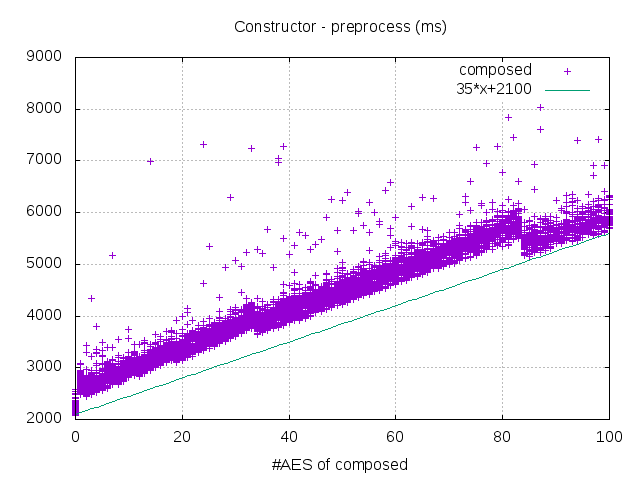
\includegraphics[width=\textwidth]{const_preprocess_plots}
        \caption{}
        \label{preprocess composed}
    \end{subfigure}
    \begin{subfigure}[t]{0.3\textwidth}
        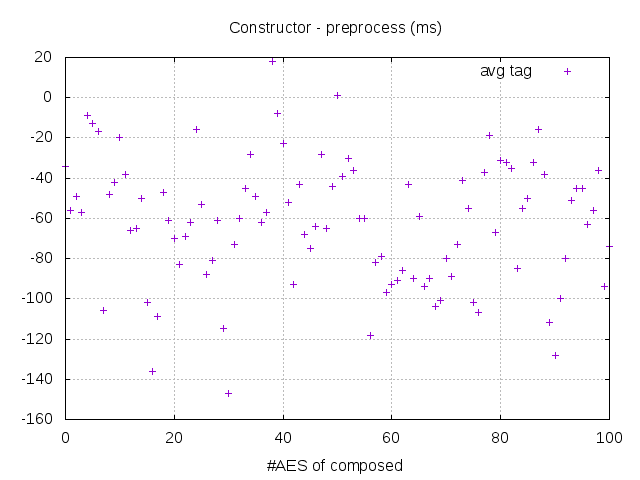
\includegraphics[width=\textwidth]{const_preprocess_avg}
        \caption{}
        \label{preprocess tag}
    \end{subfigure}
    \begin{subfigure}[t]{0.3\textwidth}
        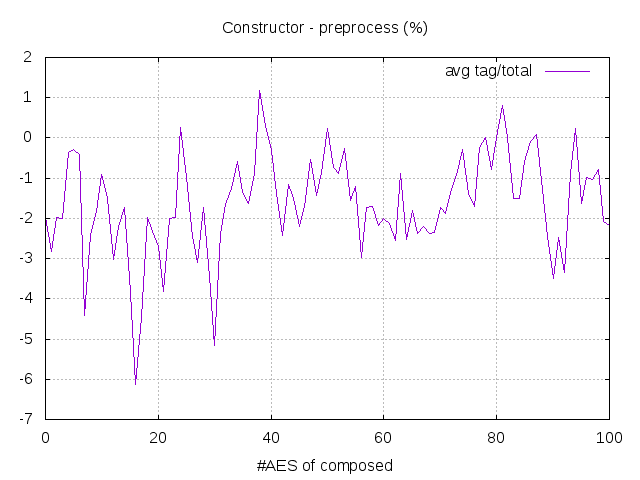
\includegraphics[width=\textwidth]{const_preprocess_frac}
        \caption{}
        \label{preprocess frac}
    \end{subfigure}
    \caption{The preprocess phase}
\end{figure}

In figure \ref{preprocess composed} we see that the preprocessing time of the composed circuit is approximate linear to the number of $C_A$ sub-circuits. We also see that the total time used preprocessing starts around 2-3 seconds without any $C_A$'s and goes up to between 6 to 7 seconds with 100 $C_A$ sub-circuits. The line plotted is an approximation for a lower bound which will be used to calculate an overall upper bound for $C_T$ of the complete evaluation after the six phases. 
Then looking at figure \ref{preprocess tag} we see that the most of the plots are below 0. This implies that the $C_T$ part of $C_{ITA}$ is so small that it is not practically measurable. 
In figure \ref{preprocess frac} is seen that the fraction of time used preprocessing the $C_T$ part of $C_{ITA}$ is minimal and below 1\% for all the composed circuits.

%SOLDER
\begin{figure}[h]
    \centering
    \begin{subfigure}[t]{0.3\textwidth}
        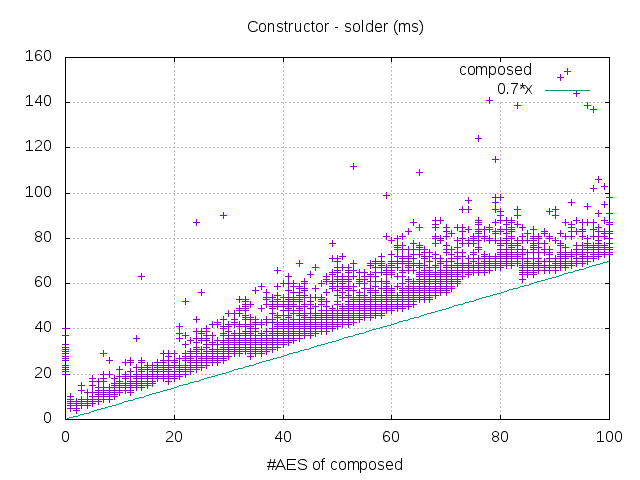
\includegraphics[width=\textwidth]{const_solder_plots}
        \caption{}
        \label{solder composed const}
    \end{subfigure}
    \begin{subfigure}[t]{0.3\textwidth}
        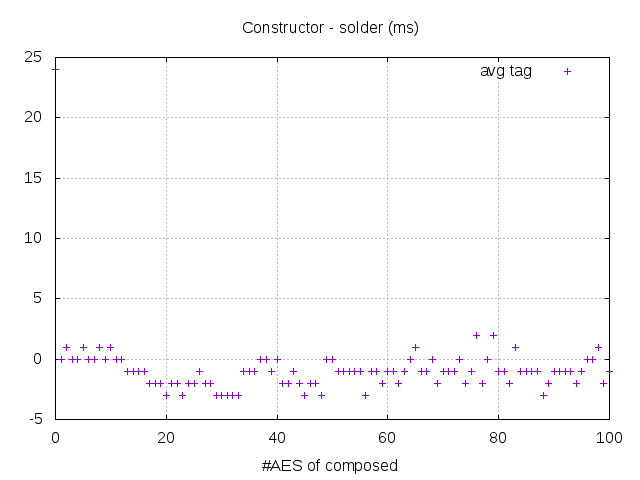
\includegraphics[width=\textwidth]{const_solder_avg}
        \caption{}
        \label{solder tag const}
    \end{subfigure}
    \begin{subfigure}[t]{0.3\textwidth}
        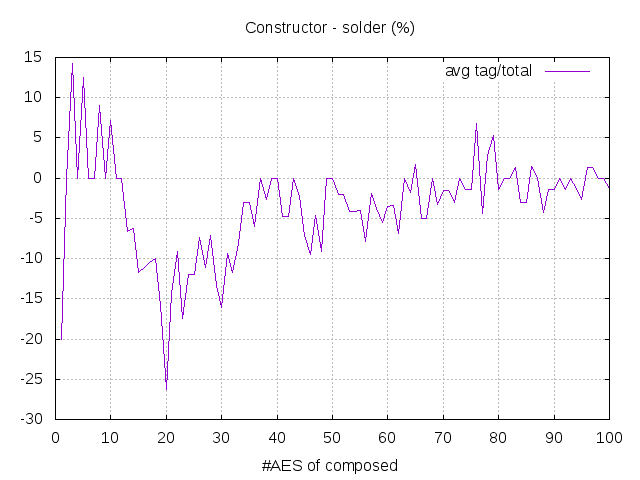
\includegraphics[width=\textwidth]{const_solder_frac}
        \caption{}
        \label{solder frac const}
    \end{subfigure}

    \begin{subfigure}[t]{0.3\textwidth}
        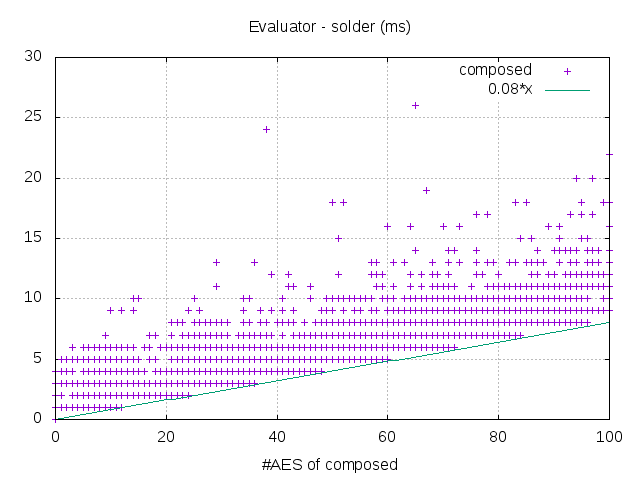
\includegraphics[width=\textwidth]{eval_solder_plots}
        \caption{}
        \label{solder composed eval}
    \end{subfigure}
    \begin{subfigure}[t]{0.3\textwidth}
        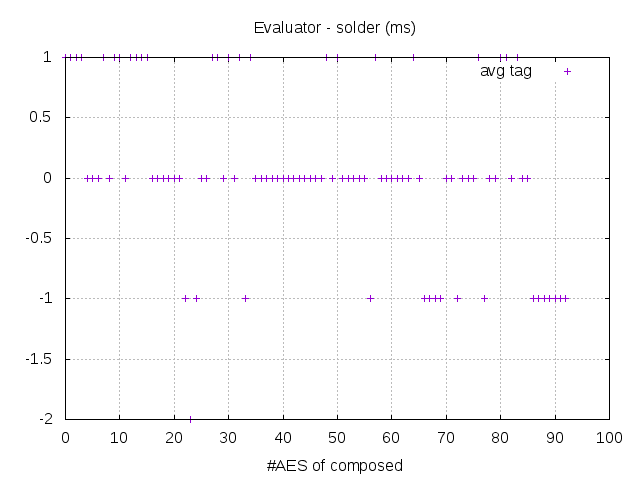
\includegraphics[width=\textwidth]{eval_solder_avg}
        \caption{}
        \label{solder tag eval}
    \end{subfigure}
    \begin{subfigure}[t]{0.3\textwidth}
        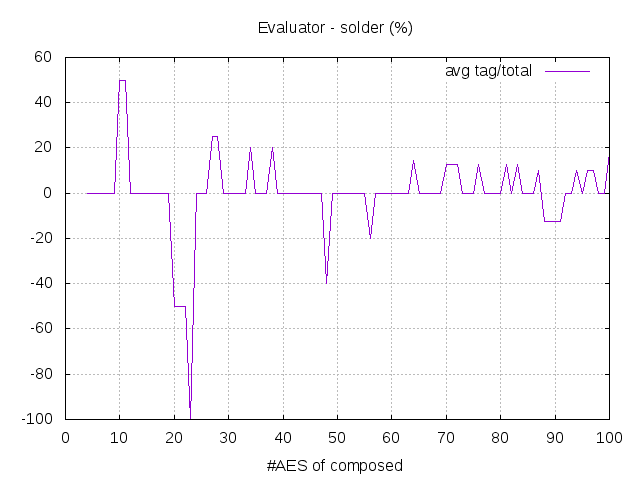
\includegraphics[width=\textwidth]{eval_solder_frac}
        \caption{}
        \label{solder frac eval}
    \end{subfigure}
    \caption{The soldering phase}
    \label{solder}
\end{figure}

The next phase timed in the experiment was the solder phase.
In this phase of the execution we see a difference between the two parties. In the figure \ref{solder} we see that both \ref{solder composed const} and \ref{solder composed eval} has plots that approximates a linear increasing function. The difference between the two plots is close to a factor 10 on the slope. Here we see one of the difference in how the framework handles the two parties. If we then look at the average time used on $C_T$ in the plots in figure \ref{solder tag const} and \ref{solder tag eval} we see that this is a constant less than 1. Which gives us the fraction seen in \ref{solder frac const} and \ref{solder frac eval} which is decreasing on the spikes over the number of $C_A$'s in $C_{ITA}$. We see that these spikes is going towards something smaller and smaller.

%PREPARE
\begin{figure}[h]
    \centering
    \begin{subfigure}[t]{0.3\textwidth}
        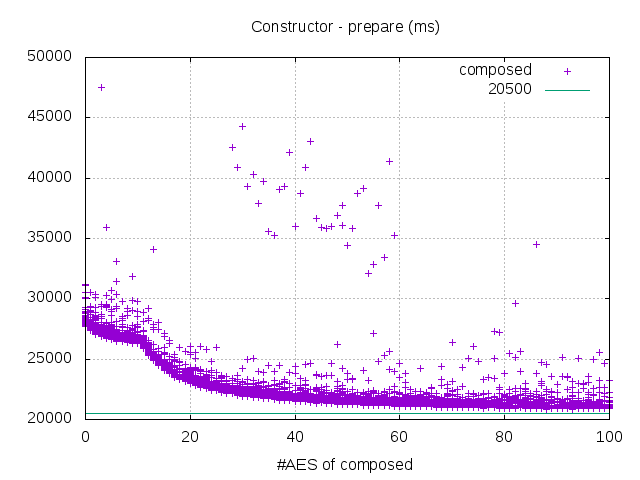
\includegraphics[width=\textwidth]{const_prepare_plots}
        \caption{}
        \label{prepare composed}
    \end{subfigure}
    \begin{subfigure}[t]{0.3\textwidth}
        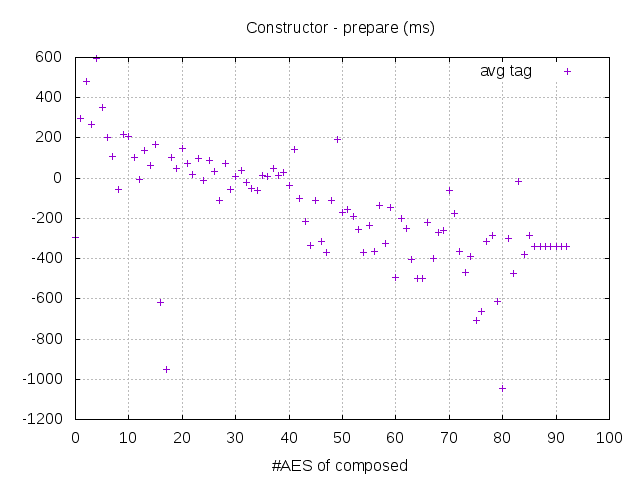
\includegraphics[width=\textwidth]{const_prepare_avg}
        \caption{}
        \label{prepare tag}
    \end{subfigure}
    \begin{subfigure}[t]{0.3\textwidth}
        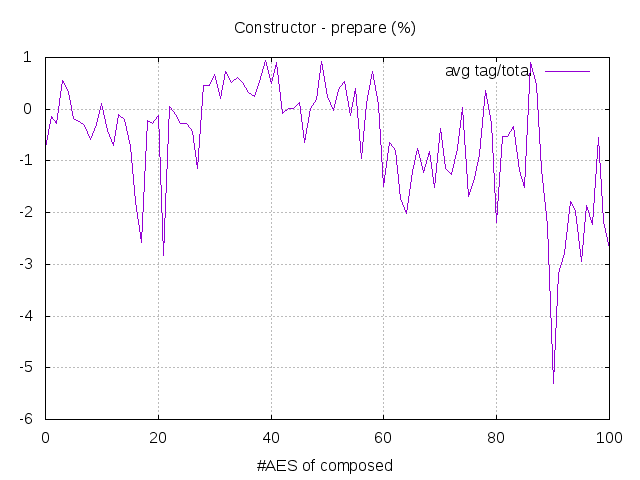
\includegraphics[width=\textwidth]{const_prepare_frac}
        \caption{}
        \label{prepare frac}
    \end{subfigure}
    \caption{The prepare phase}
\end{figure}

In the prepare phase which was the next phase timed in the evaluation the two parties plots are close to equivalent once again. This time we see that the time used on the composed circuit in figure \ref{prepare composed} approximates a hyperbola that is going towards 20 as the number of $C_A$'s increases. This is because the framework is optimized to work on "big circuits".
Then looking at the plots for the average time in figure \ref{prepare tag} we see that all the plots are below 200 ms, and maybe the average is slightly decreasing. But in worst case it is a constant less than 200 ms.

This results in a fraction of time used on $C_T$ that is in worst case is constant. Looking at figure \ref{prepare frac} it looks like it might be slightly decreasing. Again we see that many parts of the graph is below 0 which tells us that the time used on the $C_T$ part is small compared to the time used on $C_{ITA}$. We see that the graph for the fraction is below 1\% for all the experiments.

%EVALUATE
\begin{figure}[h]
    \centering
    \begin{subfigure}[t]{0.3\textwidth}
        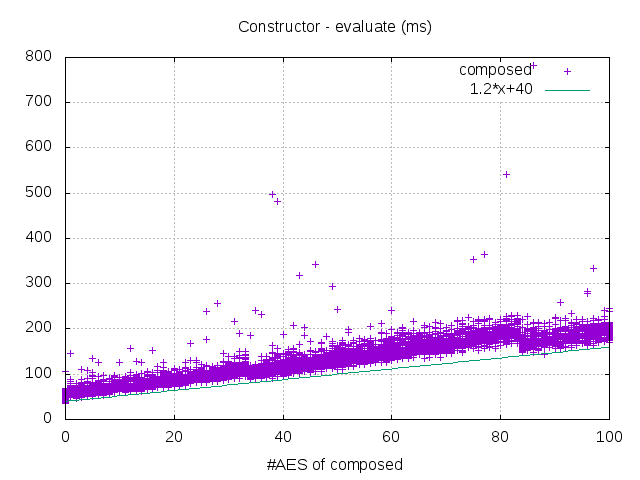
\includegraphics[width=\textwidth]{const_eval_plots}
        \caption{}
        \label{eval composed}
    \end{subfigure}
    \begin{subfigure}[t]{0.3\textwidth}
        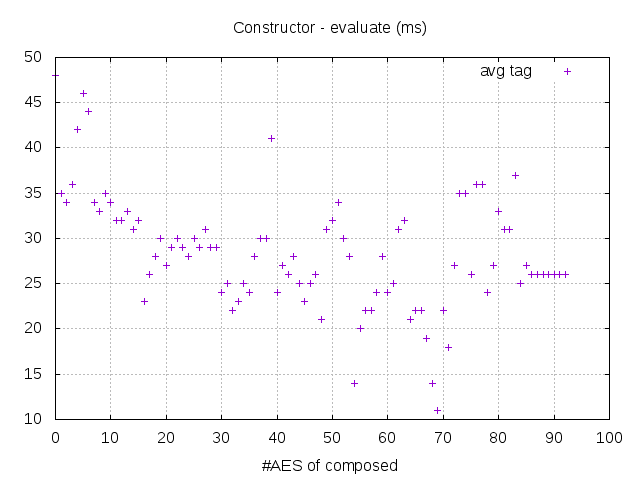
\includegraphics[width=\textwidth]{const_eval_avg}
        \caption{}
        \label{eval tag}
    \end{subfigure}
    \begin{subfigure}[t]{0.3\textwidth}
        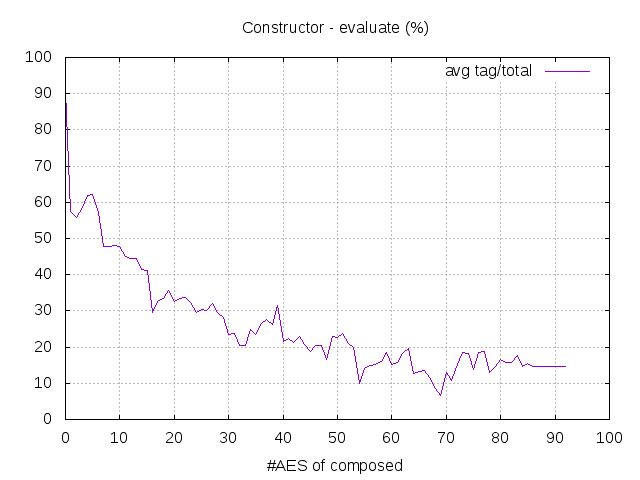
\includegraphics[width=\textwidth]{const_eval_frac}
        \caption{}
        \label{eval frac}
    \end{subfigure}
    \caption{The evaluation phase}
\end{figure}

The next phase timed was the evaluation phase.
Once again the two parties are similar when looking at the plots. Here we see that the time used on $C_{ITA}$ is approximate linear increasing as shown in figure \ref{eval composed}. When we look at the average time used on $C_T$ in figure \ref{eval tag} we see that it once again looks like it is linear and slightly decreasing. This results in the fraction we see in figure \ref{eval frac}. Here it is clear that the fraction of time used on the tag part is decreasing and it looks like it is approximating a constant that is around 10\% of $C_{ITA}$.

%DECODE
\begin{figure}[h]
    \centering
    \begin{subfigure}[t]{0.3\textwidth}
        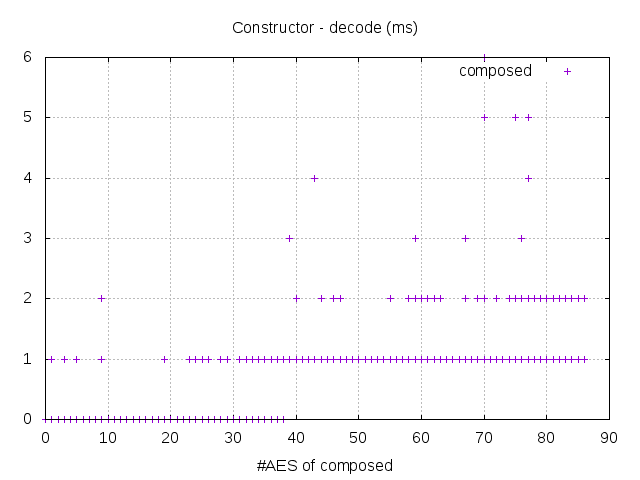
\includegraphics[width=\textwidth]{const_decode_plots}
        \caption{}
        \label{decode composed const}
    \end{subfigure}
    \begin{subfigure}[t]{0.3\textwidth}
        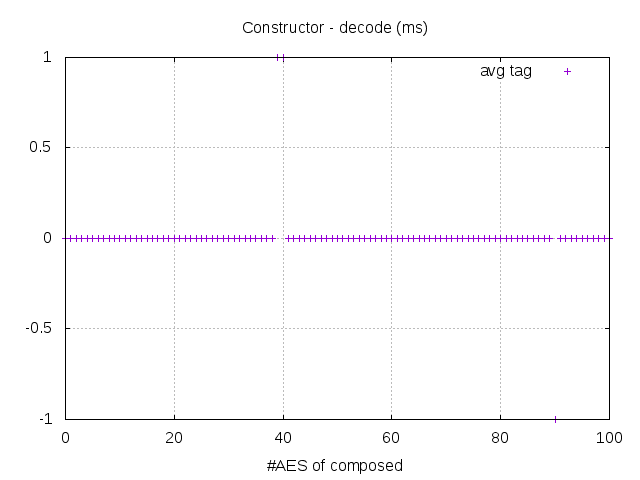
\includegraphics[width=\textwidth]{const_decode_avg}
        \caption{}
        \label{decode tag const}
    \end{subfigure}
    \begin{subfigure}[t]{0.3\textwidth}
        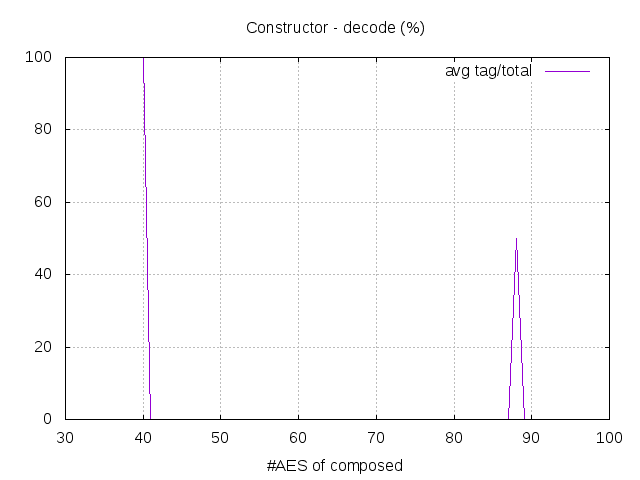
\includegraphics[width=\textwidth]{const_decode_frac}
        \caption{}
        \label{decode frac const}
    \end{subfigure}

    \begin{subfigure}[t]{0.3\textwidth}
        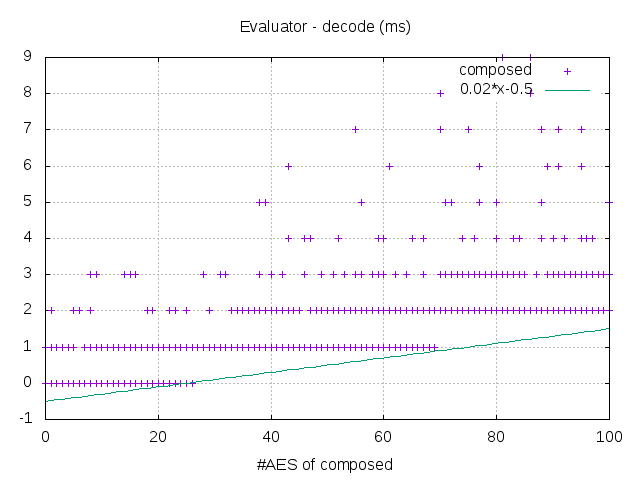
\includegraphics[width=\textwidth]{eval_decode_plots}
        \caption{}
        \label{decode composed eval}
    \end{subfigure}
    \begin{subfigure}[t]{0.3\textwidth}
        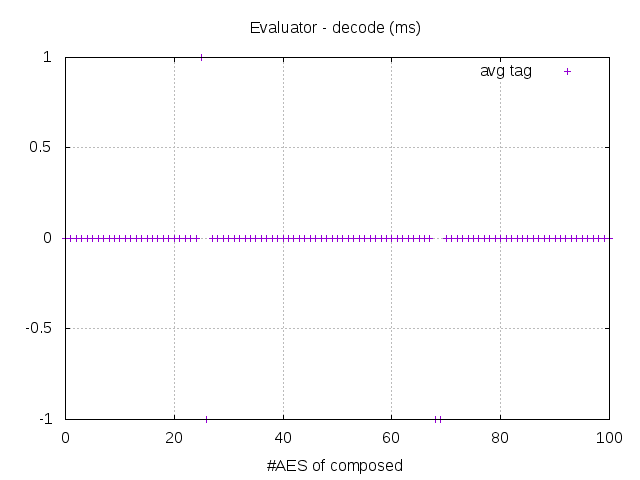
\includegraphics[width=\textwidth]{eval_decode_avg}
        \caption{}
        \label{decode tag eval}
    \end{subfigure}
    \begin{subfigure}[t]{0.3\textwidth}
        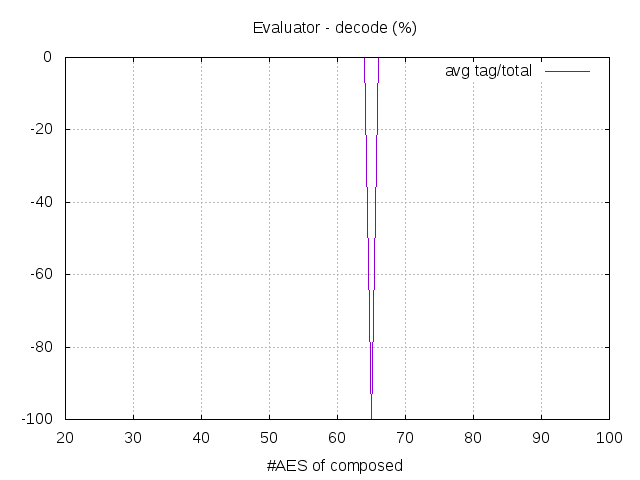
\includegraphics[width=\textwidth]{eval_decode_frac}
        \caption{}
        \label{decode frac eval}
    \end{subfigure}
    \caption{The decode phase}
\end{figure}

The last phase timed in the experiments was the decode phase.
%\todo{Describe the decode phase}
In this phase we do not see the exact same results at both parties. But in general it looks like the plots in both \ref{decode composed const} and \ref{decode composed eval} are nearly identical and linear increasing. From \ref{decode tag const} and \ref{decode tag eval} we see that the average time used on the tag part is constant and negligible. The same goes for the fraction, as seen in \ref{decode frac const} and \ref{decode frac eval}.

%\todo{Describe the overall results, total}
\bigskip
Summing up on all these plots to calculate the fraction of the time used on the $C_T$ part of $C_{ITA}$ dependent on the number of $C_A$ sub-circuits. We get the plot in figure \ref{total frac} from the function $\frac{300}{36x+22500}$ which shows as an upper bound on time used on $C_T$ of $C_{ITA}$ is approaching 0 as the amount of $C_A$'s increases.

\begin{figure}[h]
    \centering
    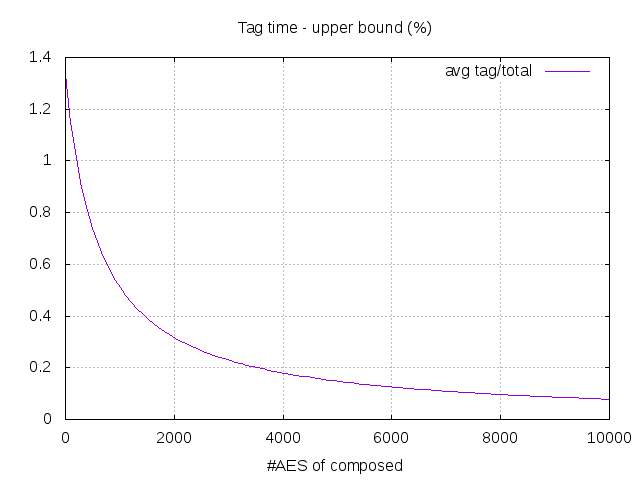
\includegraphics[width=0.5\textwidth]{total_frac}
    \caption{Total tag fraction of composed, $\frac{300}{36x+22500}$}
    \label{total frac}
\end{figure}

The plot in figure \ref{total frac} has been constructed by using the lower bound plotted in the different figures for $C_{ITA}$ and an upper bound for the average of the $C_T$ times. These numbers has been summed and the fraction of time used on $C_T$ has been calculated as an upper bound.

In the next section I will discuss the problems that I have encountered during the experiments and what could have been done differently.

\subsection{Discussion}
%DISCUSSION - optimizing results

In this section I will discuss some of the problems with the way the experiment was done and how that have effected the outcome the outcome.

First of all returning to the result in figure \ref{total frac}. Assuming that one wants that the tag fraction of the composed circuit is below 1\% then we need to have more the 208 $C_A$ subcircuits. On the laptop where the experiments was done a test run with 1000 $C_A$'s was done and completed without problems. But a circuit with 208 $C_A$ subcircuits is a big circuit with 7+ million gates. I do not know if such a "big circuit" is used for any computation in a multiparti setting.

\bigskip
Then focusing on what could have been done to make the results more precise.
In the plots used to calculate the plots of figure \ref{total frac} some things could have been done differently to make plots more precise. First of all the framework used did not have the possibility to time each sub-circuit separately such that the time used on $C_T$ could be timed such that I would not have had negative time plots. Because of the way the framework worked I needed to run two separate composed circuits one with and one without the $C_T$ part and then calculate an average and subtract them from each other to get an average of $C_T$'s part of $C_{ITA}$. This should clearly not be possible but can be observed as the $C_T$ part of $C_{ITA}$ can be ignored as it is so small compared to $C_{ITA}$ that it is not measurable. 

This problem could possibly have been avoided or at least smaller if I had used a dedicated device instead of using my person laptop. To overcome the problem with using computing resources on other computing tasks while running the experiments most of the experiments was don during nighttime. This was done to neglect the possibility of the computation having some I/O wait time, such that the timing was a precise a possible.

In the calculations I have use an average on the timing and the calculation of the total. Therefore there can be some offset to the results that could have been avoided if a more correct mathematical statistical method had been used.

\bigskip
In the last part I will try to sum up on the expectations and the outcome of the experiments.

%CONCLUTION
\section{Conclusion}
%\todo{What was the hypothesis}
In the paper \cite{fosc} they state that the addition of an AMD code to the proposed framework is minimal. Therefore we expected that the overhead of the tag added in the experiments according to the section \ref{tag-circuit} about the tag circuit would be minimal and probably negligible as the number of AES circuits grow.

%\todo{What was the conclution}
From the results in the section \ref{results} and in figure \ref{total frac} summing the overall result. We see that the addition of this type of tag is minimal. We get that the time used on the tag part is less than 1.4\% and declining from there towards negligibly. 
From the results we also see that the most of the time is used on preparing the evaluation of the circuit. Here the fraction of time used on the TAG is less than 1\%. The parts where the tag uses the highest fraction of time is in the evaluation and solder phase. But we see that both of these phases do not take very long time compared to the prepare and preprocessing phase where the fraction of time used on the tag is less than 1\%. That is why overall the tag is negligible. For more precise evaluation of conclusion see the section \ref{results}.


\pagebreak
%BIB
\bibliography{report}
\bibliographystyle{alpha}

\appendix

\section{Data}
\label{data appendix}
All data generated and used in this report can be found at \href{https://github.com/cbobach/mpc-outsourcing}{GitHub}\footnote{All the data files and plots can be found here: https://github.com/cbobach/mpc-outsourcing}. The data was generated using a framework 'duplo' which is an ongoing PhD. project by Roberto Trifiletti, which is not public at the moment of writing. All data was collected via a local-host on a standard laptop with a i5-4210U, 1.7GHz processor, 12GB 1600MHz ram and 6.0Gb/s ssd running Ubuntu 16.10.

The framework consist of 6 different phases, setup, preprocess, solder, prepare, evaluate and decode. Each of these except setup timed are plotted in the following figures. Each of the subsections contains six plots, the first three are form the constructor and the next three are from the evaluator.

For conclusion on the different plots and the hypothesis can be read in the abstract and conclusion.

\begin{figure}[h]
    \centering
    \begin{subfigure}[t]{0.3\textwidth}
        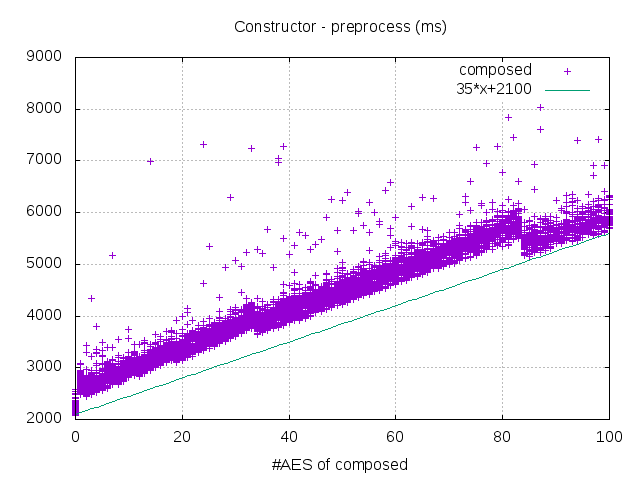
\includegraphics[width=\textwidth]{const_preprocess_plots}
        \caption{}
        \label{data const preprocess composed}
    \end{subfigure}
    \begin{subfigure}[t]{0.3\textwidth}
        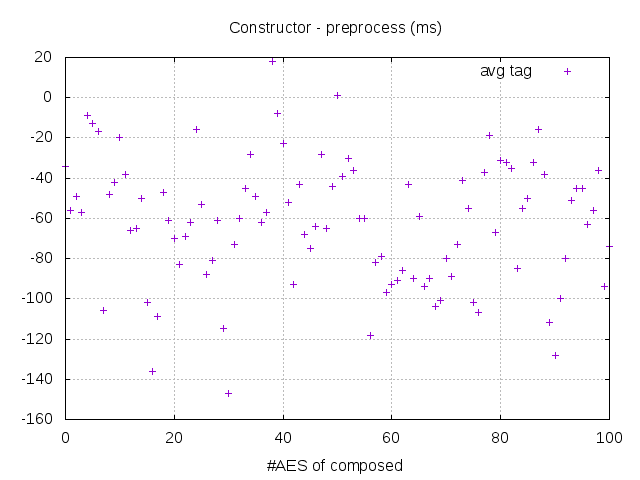
\includegraphics[width=\textwidth]{const_preprocess_avg}
        \caption{}
        \label{data const preprocess avg}
    \end{subfigure}
    \begin{subfigure}[t]{0.3\textwidth}
        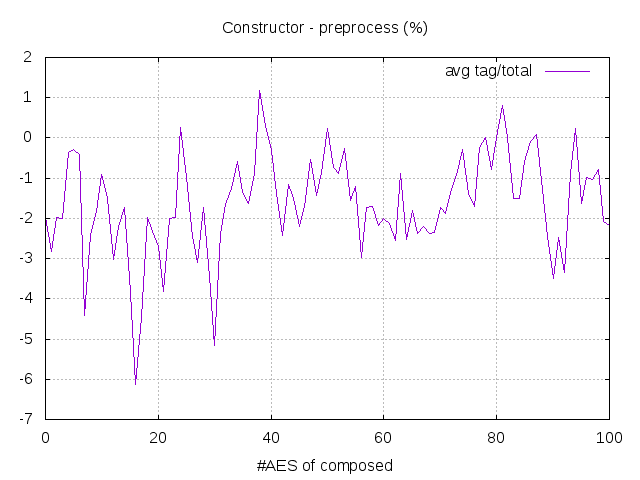
\includegraphics[width=\textwidth]{const_preprocess_frac}
        \caption{}
        \label{data const preprocess frac}
    \end{subfigure}

    \begin{subfigure}[t]{0.3\textwidth}
        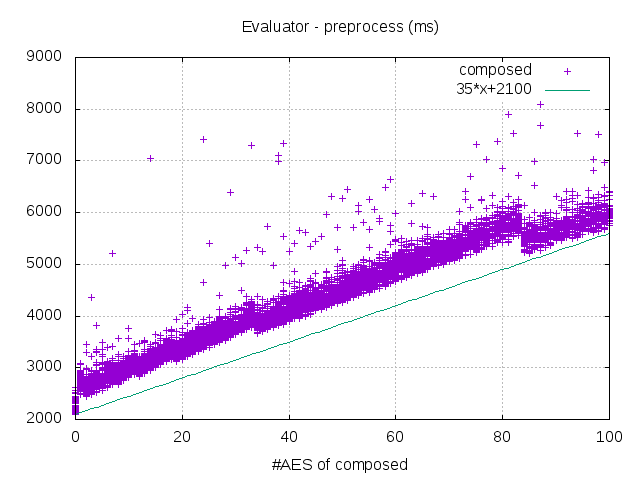
\includegraphics[width=\textwidth]{eval_preprocess_plots}
        \caption{}
        \label{data eval preprocess composed}
    \end{subfigure}
    \begin{subfigure}[t]{0.3\textwidth}
        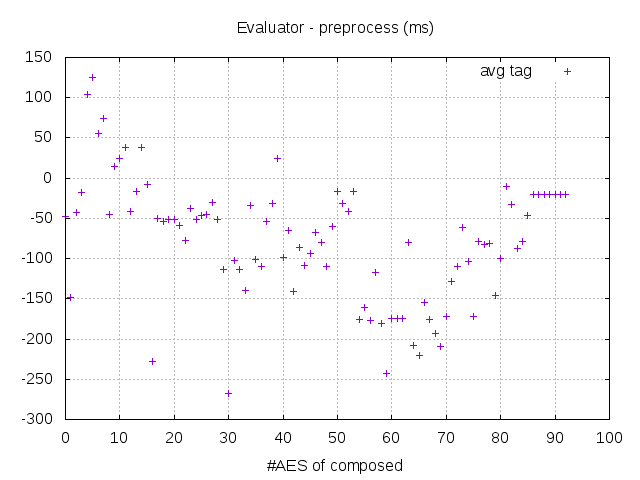
\includegraphics[width=\textwidth]{eval_preprocess_avg}
        \caption{}
        \label{data eval preprocess avg}
    \end{subfigure}
    \begin{subfigure}[t]{0.3\textwidth}
        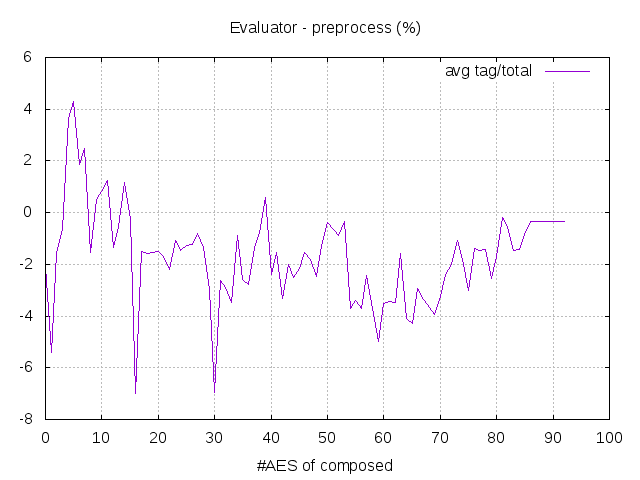
\includegraphics[width=\textwidth]{eval_preprocess_frac}
        \caption{}
        \label{data eval preprocess frac}
    \end{subfigure}
    \caption{The preprocess phase is run on one instance of the ID- and TAG-circuit, while it is run on multiple instances of the AES-circuit. \ref{data const prerocess composed} Constructor, total time used on the composed circuit. \ref{data const preprocess avg} Constructor, average time used on tag part. \ref{data eval preprocess composed} Constructor, fraction of time used on tag part. \ref{data eval preprocess composed} Evaluator, total time used on the composed circuit. \ref{data eval preprocess avg} Evaluator, average time used on tag part. \ref{data eval preprocess frac} Evaluator, fraction of time used on tag part.}
\end{figure}

\begin{figure}[h]
    \centering
    \begin{subfigure}[t]{0.3\textwidth}
        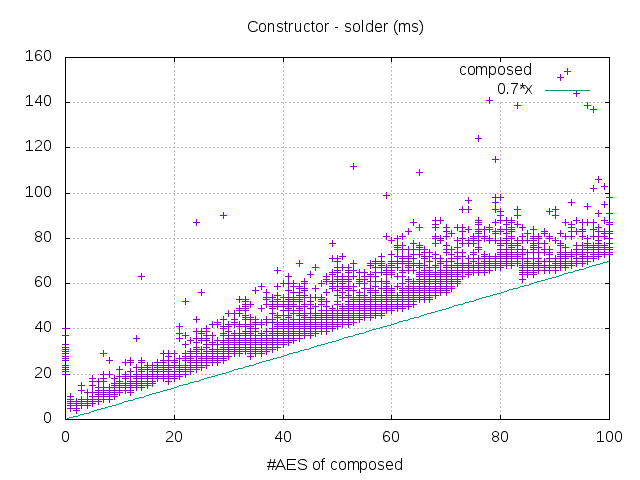
\includegraphics[width=\textwidth]{const_solder_plots}
        \caption{}
        \label{data const solder composed}
    \end{subfigure}
    \begin{subfigure}[t]{0.3\textwidth}
        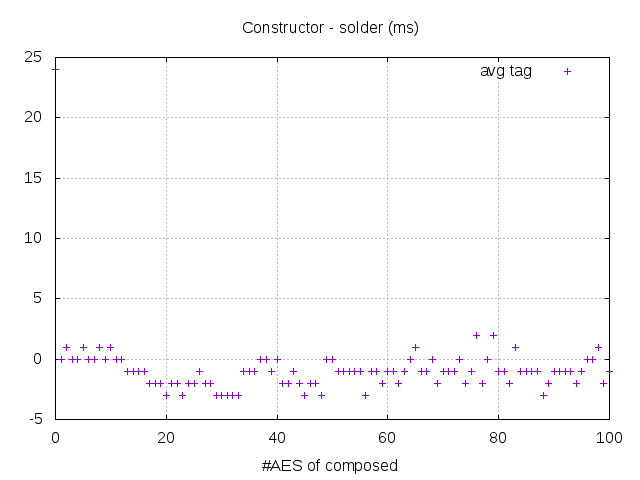
\includegraphics[width=\textwidth]{const_solder_avg}
        \caption{}
        \label{data const solder avg}
    \end{subfigure}
    \begin{subfigure}[t]{0.3\textwidth}
        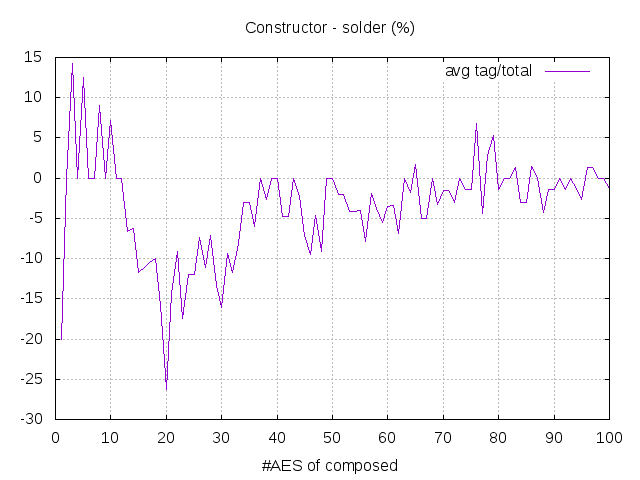
\includegraphics[width=\textwidth]{const_solder_frac}
        \caption{}
        \label{data const solder frac}
    \end{subfigure}

    \begin{subfigure}[t]{0.3\textwidth}
        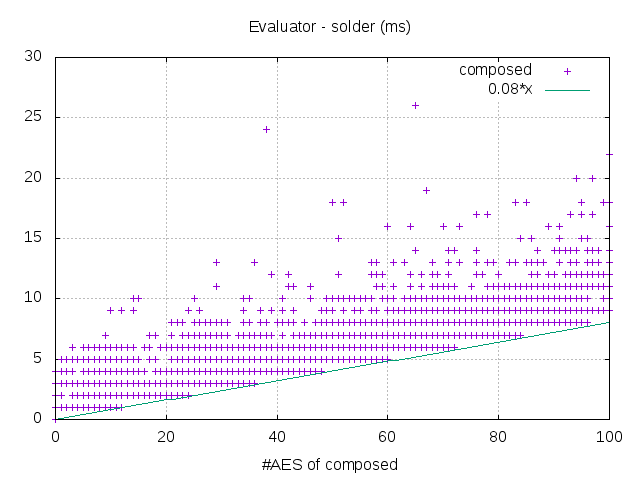
\includegraphics[width=\textwidth]{eval_solder_plots}
        \caption{}
        \label{data eval solder composed}
    \end{subfigure}
    \begin{subfigure}[t]{0.3\textwidth}
        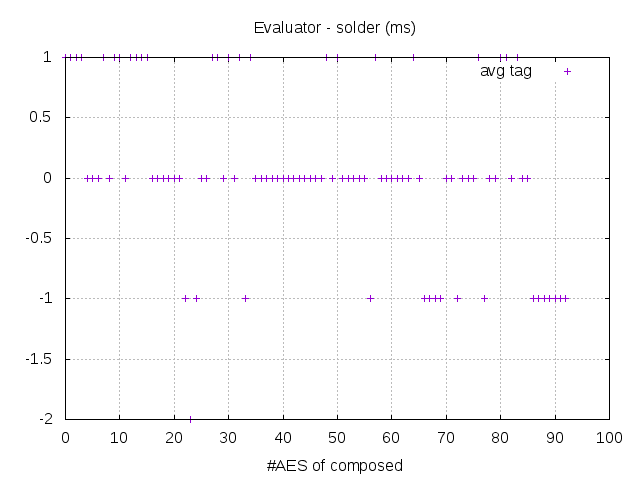
\includegraphics[width=\textwidth]{eval_solder_avg}
        \caption{}
        \label{data eval solder avg}
    \end{subfigure}
    \begin{subfigure}[t]{0.3\textwidth}
        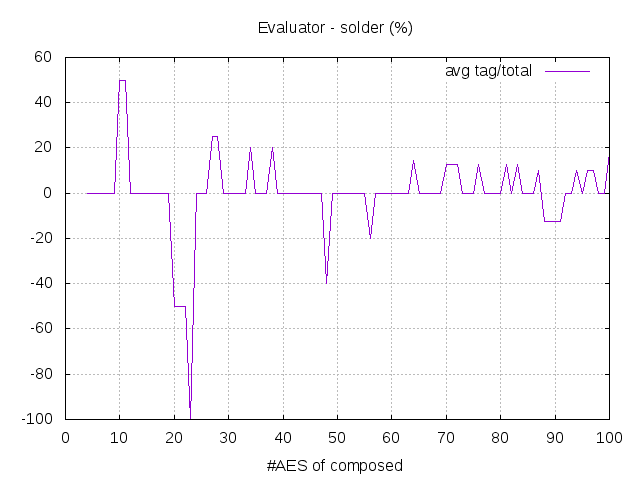
\includegraphics[width=\textwidth]{eval_solder_frac}
        \caption{}
        \label{data eval solder frac}
    \end{subfigure}
    \caption{The solder phase is where the preprocessed circuits are composed into one circuit. \ref{data const solder composed} Constructor, total time used on the composed circuit. \ref{data const solder avg} Constructor, average time used on tag part. \ref{data const solder frac} Constructor, fraction of time used on tag part. \ref{data eval solder composed} Evaluator, total time used on the composed circuit. \ref{data eval solder avg} Evaluator, average time used on tag part. \ref{data eval solder frac} Evaluator, fraction of time used on tag part.}
\end{figure}

\begin{figure}[h]
    \centering
    \begin{subfigure}[t]{0.3\textwidth}
        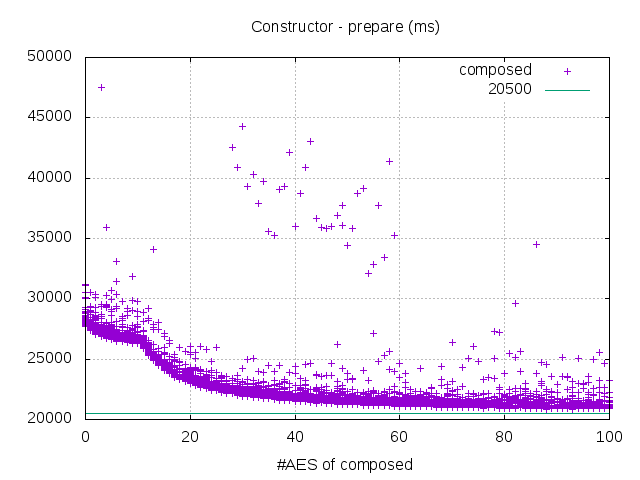
\includegraphics[width=\textwidth]{const_prepare_plots}
        \caption{}
        \label{data const prepare composed}
    \end{subfigure}
    \begin{subfigure}[t]{0.3\textwidth}
        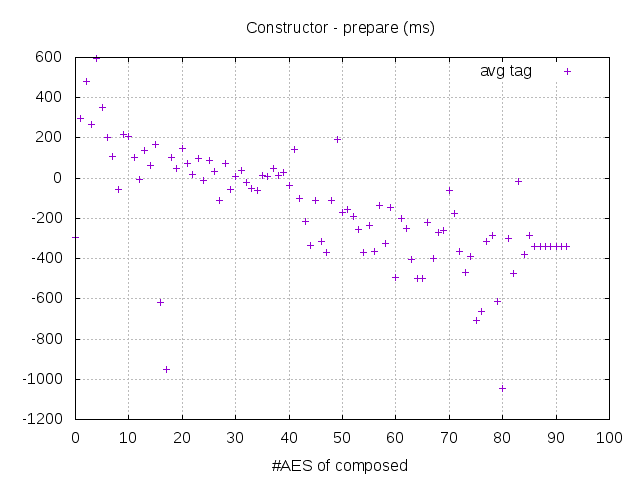
\includegraphics[width=\textwidth]{const_prepare_avg}
        \caption{}
        \label{data const prepare tag}
    \end{subfigure}
    \begin{subfigure}[t]{0.3\textwidth}
        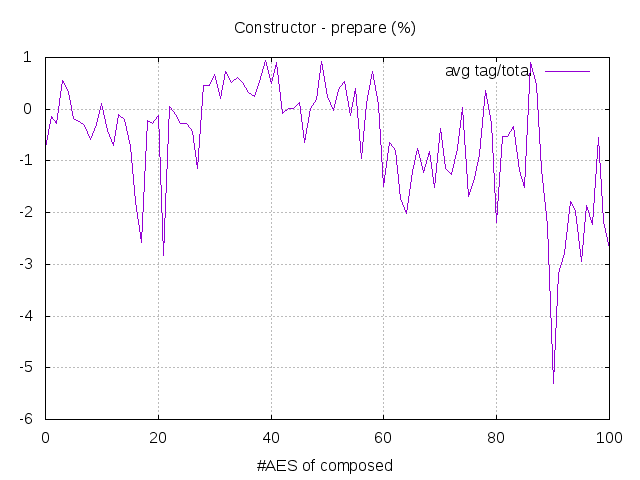
\includegraphics[width=\textwidth]{const_prepare_frac}
        \caption{}
        \label{data const prepare frac}
    \end{subfigure}

    \begin{subfigure}[t]{0.3\textwidth}
        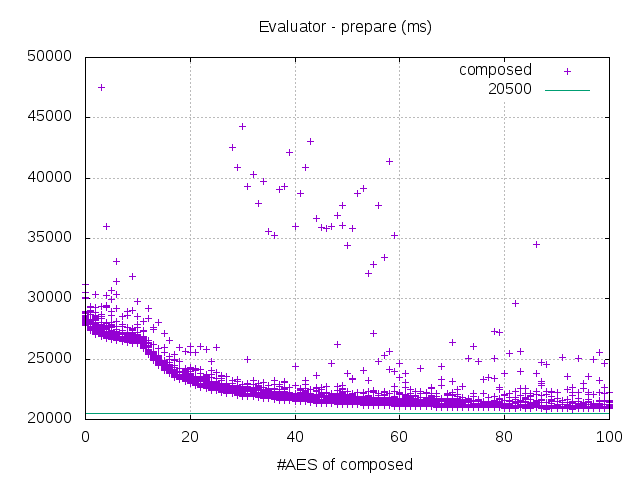
\includegraphics[width=\textwidth]{eval_prepare_plots}
        \caption{}
        \label{data eval prepare composed}
    \end{subfigure}
    \begin{subfigure}[t]{0.3\textwidth}
        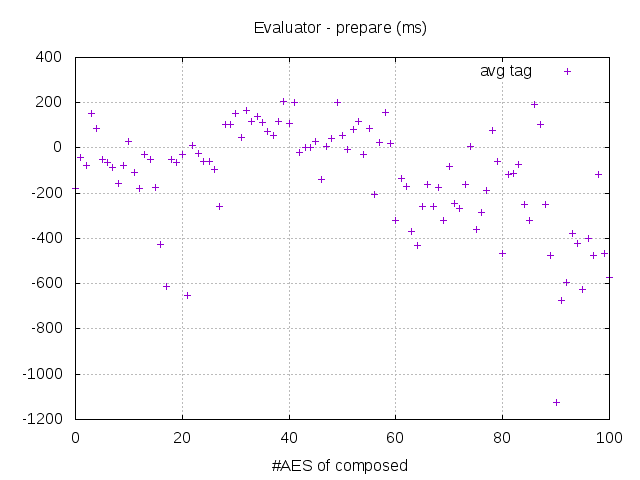
\includegraphics[width=\textwidth]{eval_prepare_avg}
        \caption{}
        \label{data eval prepare tag}
    \end{subfigure}
    \begin{subfigure}[t]{0.3\textwidth}
        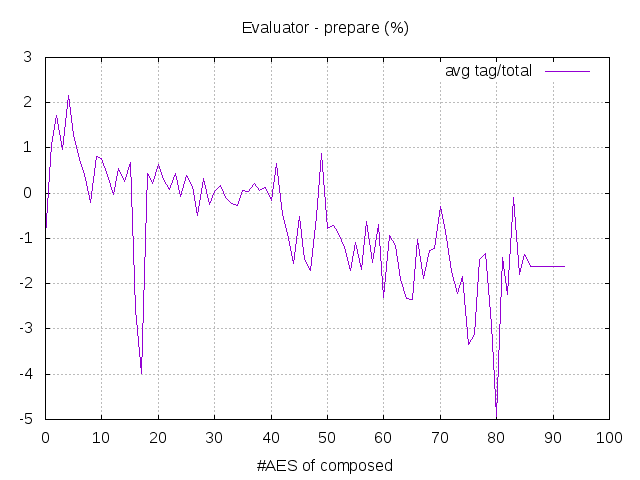
\includegraphics[width=\textwidth]{eval_prepare_frac}
        \caption{}
        \label{data eval prepare frac}
    \end{subfigure}
    \caption{In the prepare phase the composed circuit is prepared for evaluation. \ref{data const prepare composed} Constructor, total time used on the composed circuit. \ref{data const prepare tag} Constructor, average time used on tag part. \ref{data const prepare frac} Constructor, fraction of time used on tag part. \ref{data eval prepare composed} Evaluator, total time used on the composed circuit. \ref{data eval prepare tag} Evaluator, average time used on tag part. \ref{data eval prepare frac} Evaluator, fraction of time used on tag part.}
\end{figure}

\begin{figure}[h]
    \centering
    \begin{subfigure}[t]{0.3\textwidth}
        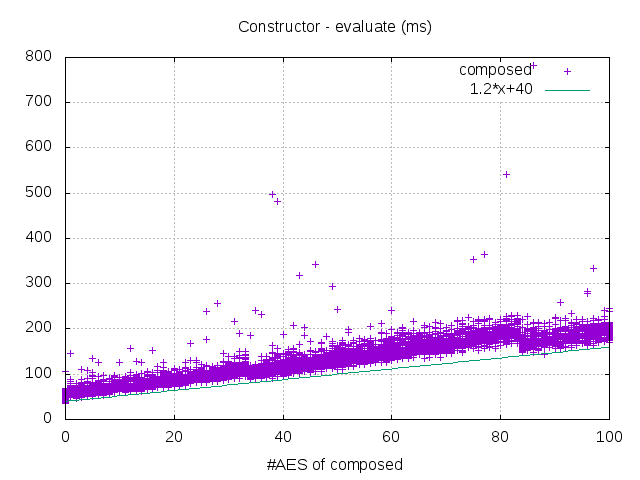
\includegraphics[width=\textwidth]{const_eval_plots}
        \caption{}
        \label{data const eval composed}
    \end{subfigure}
    \begin{subfigure}[t]{0.3\textwidth}
        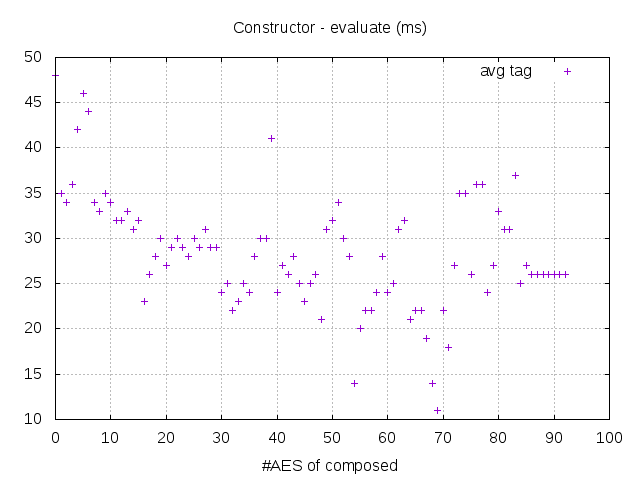
\includegraphics[width=\textwidth]{const_eval_avg}
        \caption{}
        \label{data const eval tag}
    \end{subfigure}
    \begin{subfigure}[t]{0.3\textwidth}
        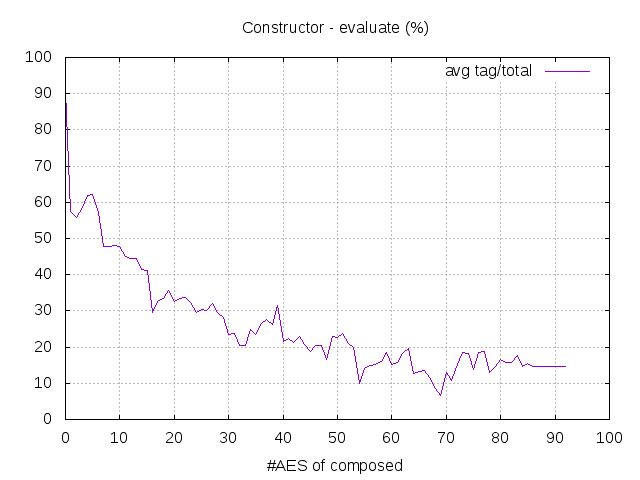
\includegraphics[width=\textwidth]{const_eval_frac}
        \caption{}
        \label{data const eval frac}
    \end{subfigure}

    \begin{subfigure}[t]{0.3\textwidth}
        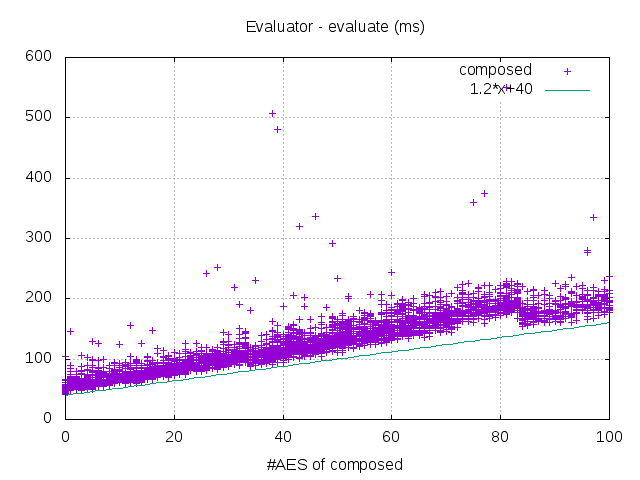
\includegraphics[width=\textwidth]{eval_eval_plots}
        \caption{}
        \label{data eval eval composed}
    \end{subfigure}
    \begin{subfigure}[t]{0.3\textwidth}
        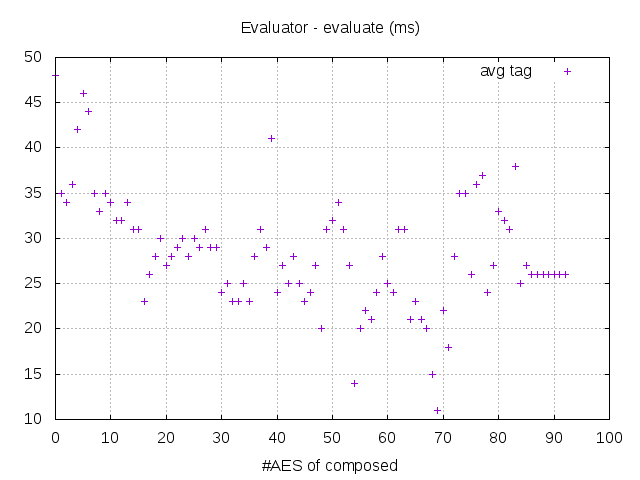
\includegraphics[width=\textwidth]{eval_eval_avg}
        \caption{}
        \label{data eval eval tag}
    \end{subfigure}
    \begin{subfigure}[t]{0.3\textwidth}
        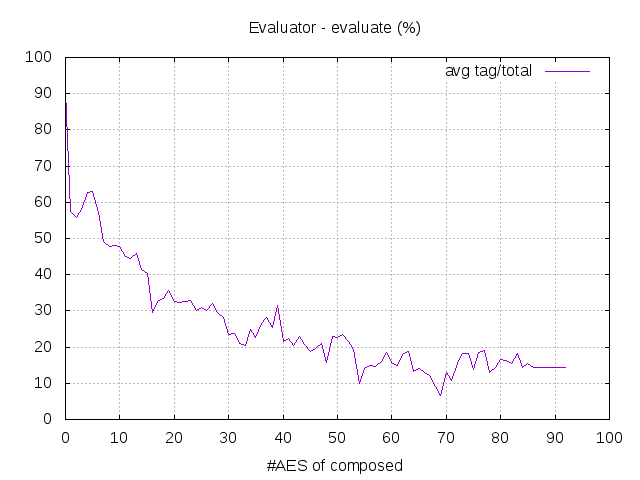
\includegraphics[width=\textwidth]{eval_eval_frac}
        \caption{}
        \label{data eval eval frac}
    \end{subfigure}
    \caption{In the evaluation phase the composed circuit is evaluated. \ref{data const eval composed} Constructor, total time used on the composed circuit. \ref{data const eval tag} Constructor, average time used on tag part. \ref{data const eval tag} Constructor, fraction of time used on tag part. \ref{data eval eval composed} Evaluator, total time used on the composed circuit. \ref{data eval eval tag} Evaluator, average time used on tag part. \ref{data eval eval frac} Evaluator, fraction of time used on tag part.}
\end{figure}

\begin{figure}[h]
    \centering
    \begin{subfigure}[t]{0.3\textwidth}
        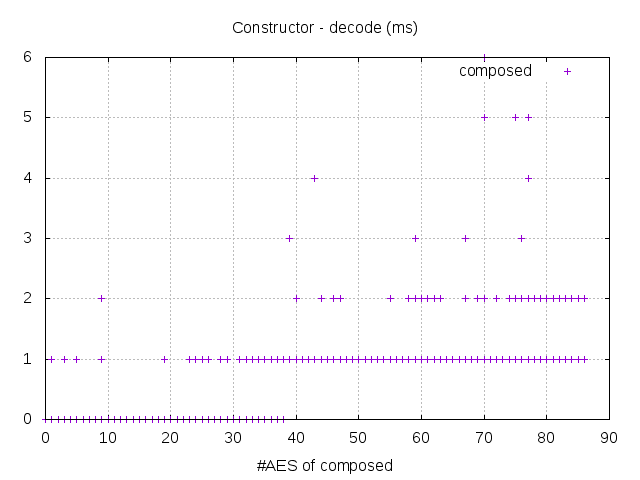
\includegraphics[width=\textwidth]{const_decode_plots}
        \caption{}
        \label{data const decode composed}
    \end{subfigure}
    \begin{subfigure}[t]{0.3\textwidth}
        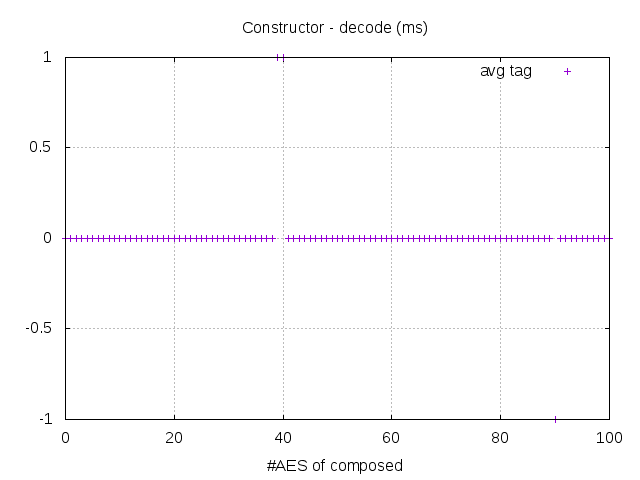
\includegraphics[width=\textwidth]{const_decode_avg}
        \caption{}
        \label{data const decode tag}
    \end{subfigure}
    \begin{subfigure}[t]{0.3\textwidth}
        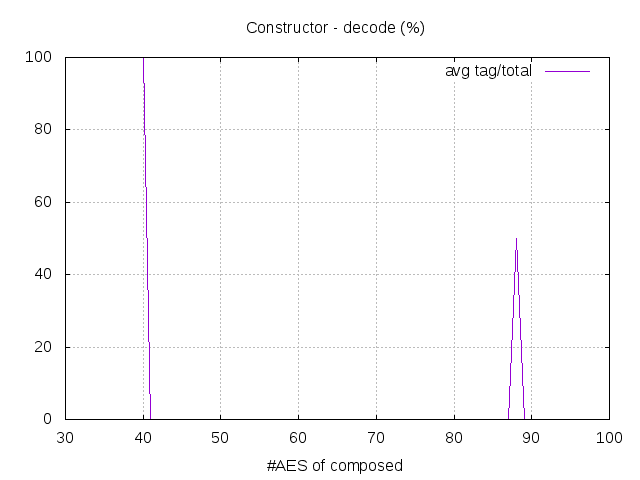
\includegraphics[width=\textwidth]{const_decode_frac}
        \caption{}
        \label{data const decode frac}
    \end{subfigure}

    \begin{subfigure}[t]{0.3\textwidth}
        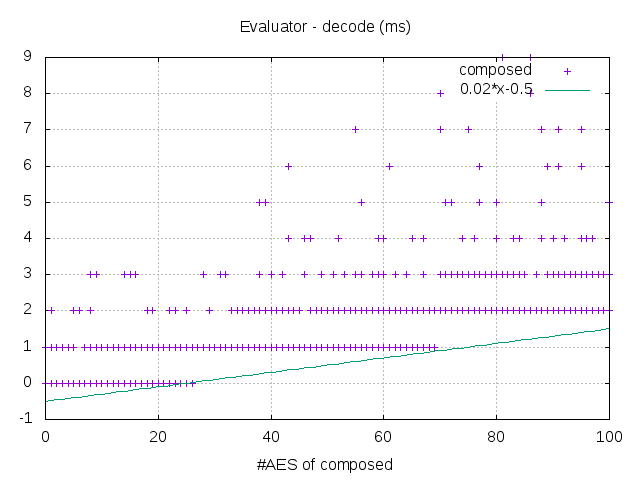
\includegraphics[width=\textwidth]{eval_decode_plots}
        \caption{}
        \label{data eval decode composed}
    \end{subfigure}
    \begin{subfigure}[t]{0.3\textwidth}
        \includegraphics[width=\textwidth]{eval_decode_avg}
        \caption{}
        \label{data eval decode tag}
    \end{subfigure}
    \begin{subfigure}[t]{0.3\textwidth}
        \includegraphics[width=\textwidth]{eval_decode_frac}
        \caption{}
        \label{data eval decode frac}
    \end{subfigure}
    \caption{In the decode phase the output from the composed circuit is decoded. \ref{data const decode composed} Constructor, total time used on the composed circuit. \ref{data const decode tag} Constructor, average time used on tag part. \ref{data const decode frac} Constructor, fraction of time used on tag part. \ref{data eval decode composed} Evaluator,  total time used on the composed circuit. \ref{data eval decode tag} Evaluator, average time used on tag part. \ref{data eval decode frac} Evaluator, fraction of time used on tag part.}
\end{figure}

\begin{figure}[h]
    \centering
    \includegraphics[width=0.5\textwidth]{total_frac}
    \caption{For the plot every line in the composed timings has been summed and a constant upper bound for all the average plots has been used to calculate the fraction. Resulting in $\frac{300}{36x+22500}$ as an upper bound on the tag fraction of the composed circuit.}
    \label{data total}
\end{figure}

\end{document}